\fillsectionornament
\section{Numerical Results}
\label{sec:54results}

\minitoc{85mm}{5}

\noindent
The following numerical experiments can be roughly divided into two parts.
First, we study interpolation errors for the test functions
to assess the effects of the hierarchical B-spline bases introduced in
\cref{chap:20sparseGrids,chap:30BSplines} on interpolation.
Second, we consider the optimality gaps $\objfun(\xoptappr) - \objfun(\xopt)$
of the calculated approximations $\xoptappr$
of the point $\xopt$ at which the objective function $\objfun$
is minimal.

\pagebreak

The results have been computed with the sparse grid toolbox \sgpp
\cite{Pflueger10Spatially},%
\footnote{%
  \url{http://sgpp.sparsegrids.org/}%
}
which has been extended in the scope of this thesis.
The new code has been written in such a way that
it is scalable and efficient, while still being maintainable and
portable \cite{Pflueger16Scalability}.



\subsection{Interpolation Error and Decay of Surpluses}
\label{sec:541interpolation}

\paragraph{Interpolation error for different test functions}

\Cref{fig:resultsInterpolationErrorTestFunctions} shows the
relative $\Ltwo$ interpolation error
$\tfrac{\normLtwo{\objfun - \sgintp}}{\normLtwo{\objfun}}$
of sparse grid interpolants $\sgintp$ to
different objective functions $\objfun$
(approximated via Monte Carlo quadrature using
$10^4$ uniformly pseudo-random samples).
The interpolation is performed on regular sparse grids of increasing levels
using hierarchical not-a-knot B-splines $\bspl[\nak]{\*l,\*i}{p}$
of degree $p = 1, 3, 5$.
As a visual aid, the plots include gray lines that indicate different
orders of convergence.

\begin{figure}
  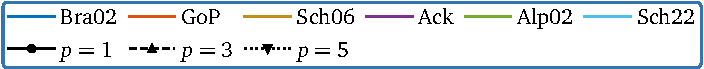
\includegraphics{resultsInterpolationLegend_1}\\[2mm]%
  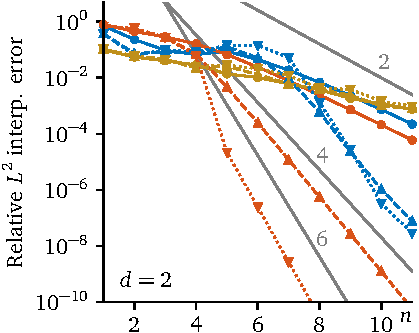
\includegraphics{resultsInterpolation_2}%
  \hfill%
  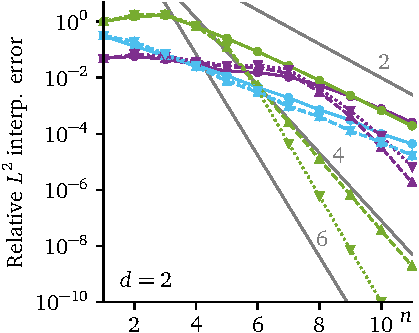
\includegraphics{resultsInterpolation_4}%
  \\[2mm]%
  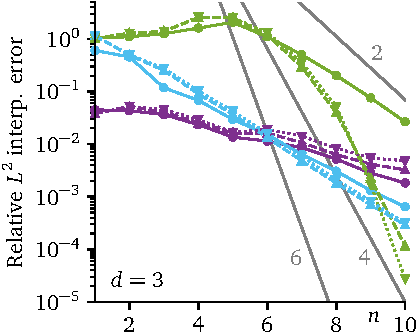
\includegraphics{resultsInterpolation_6}%
  \hfill%
  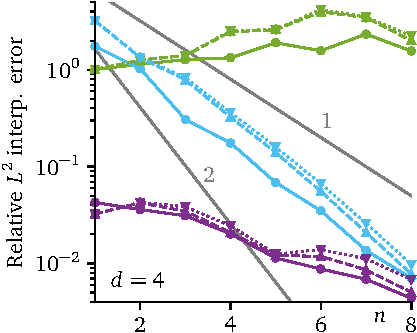
\includegraphics{resultsInterpolation_8}%
  \caption[Relative interpolation error for different test functions]{%
    Relative $\Ltwo$ interpolation error
    \vspace{-0.05em}%
    $\normLtwo{\objfun - \sgintp}/\normLtwo{\objfun}$
    for different test functions $\objfun$ \emph{(colors)}
    using hierarchical not-a-knot B-splines
    $\bspl[\nak]{\*l,\*i}{p}$ of different degrees $p$
    \emph{(line styles/markers)} on
    regular sparse grids $\regsgset{n}{d}$ of different levels $n$.%
  }%
  \label{fig:resultsInterpolationErrorTestFunctions}%
\end{figure}

It is already known that---%
if the objective function is sufficiently smooth---%
the $\Ltwo$ error of spline interpolants of degree $p$ on
$d$-dimensional regular sparse grids of level $n$
asymptotically behaves like
$\landauO{\ms{n}^{p+1} (\log_2 \ms{n}^{-1})^{d-1}}
= \landauO{2^{-(p+1)n} n^{d-1}}$ for $n \to \infty$ \cite{Sickel11Spline}.
We can numerically verify this fact easily with
\cref{fig:resultsInterpolationErrorTestFunctions},
in which we obtain the asserted orders of convergence
\pagebreak%
for the bivariate functions that are continuously differentiable.
For the functions Sch06 and Sch22, which have a non-differentiable kink,
only linear convergence can be achieved regardless of the B-spline degree.

\vspace*{\fill}

The region where the asymptotic behavior dominates largely depends
on the objective function at hand.
Functions like Bra02 and Ack with many small oscillations
require more interpolation points than ``smoother'' functions like
GoP and Alp02.
This is also the case for all functions in higher dimensionalities,
as more interpolation points are necessary to sufficiently explore the domain
(curse of dimensionality).
In \cref{fig:resultsInterpolationErrorTestFunctions}, this can already be seen
for $d \ge 3$.
This is not a consequence of employing higher-order B-splines for
the hierarchical basis.
However, it seems that higher-order B-splines lead to a slight increase
of the interpolation error in the preasymptotic range.

\pagebreak

\paragraph{Interpolation error for different basis functions}

In \cref{fig:resultsInterpolationErrorBasisFunctions},
we fix the objective function and study the influence of the choice
of hierarchical basis functions on the interpolation error.
Shown are eight types of hierarchical B-spline bases as introduced in
\cref{chap:20sparseGrids,chap:30BSplines} for the degrees $p = 1, 3, 5$.
Note that some lines exactly overlap, which is indicated in
the figure.

For $p = 1$, the non-modified bases and the modified bases coincide.
For higher degrees, the modified bases show worse results than
the corresponding non-modified versions for the same level $n$.
However, modified bases need significantly less grid points
(no boundary points),
which means that a direct comparison based on the sparse grid level $n$
is somewhat skewed.
%
In addition, we see that the not-a-knot bases coincide exactly for $p > 1$,
as they span the same space for regular and
dimensionally adaptive sparse grids.
Only with the not-a-knot boundary conditions, we obtain the true
theoretical order of convergence, which is $p + 1$ for degree $p$.
Otherwise, only quadratic convergence can be achieved regardless of $p$,
albeit with a smaller constant (offset).

\begin{SCfigure}
  \begin{minipage}{98mm}%
    \hspace*{4mm}%
    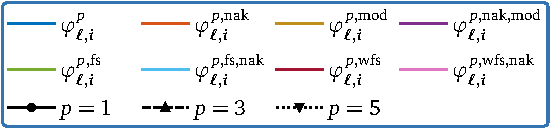
\includegraphics{resultsInterpolationLegend_2}\\[2mm]%
    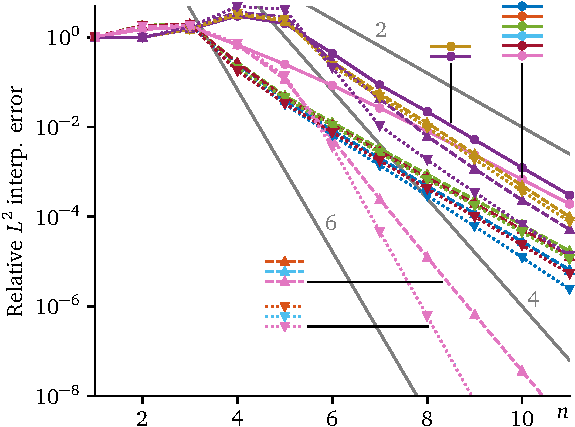
\includegraphics{resultsInterpolation_10}%
  \end{minipage}%
  \caption[Relative interpolation error for different basis functions]{%
    Relative $\Ltwo$ interpolation error
    $\normLtwo{\objfun - \sgintp}/\normLtwo{\objfun}$
    for the bivariate Alp02 function ($d = 2$)
    using different hierarchical basis functions
    $\basis{\*l,\*i}$ \emph{(colors)}
    of different degrees $p$ \emph{(line styles/markers)} and
    regular sparse grids $\regsgset{n}{d}$ of different levels $n$.\\
    The basis functions shown here involve
    standard \emph{(no superscript),}
    not-a-knot ($\mathrm{nak}$),
    modified ($\mathrm{mod}$),
    fundamental ($\mathrm{fs}$), and
    weakly fundamental ($\mathrm{wfs}$)
    splines as well as the combinations
    introduced in \cref{chap:20sparseGrids,chap:30BSplines}.%
  }%
  \label{fig:resultsInterpolationErrorBasisFunctions}%
\end{SCfigure}

\vspace*{-0.5em}

\paragraph{Pointwise interpolation error}

The importance of not-a-knot boundary conditions is also evident
from plots of the pointwise interpolation error as in
\cref{fig:resultsInterpolationErrorPointwise}.
The interpolation error grows for the standard hierarchical
B-spline basis $\bspl{\*l,\*i}{p}$
as we move towards the boundary of the domain $\clint{\*0, \*1}$,
before dropping to zero or near-zero values at or near boundary grid points.
With not-a-knot B-splines $\bspl[\nak]{\*l,\*i}{p}$,
the interpolation error is uniformly low.
For comparison, modified B-splines $\bspl[\modified]{\*l,\*i}{p}$
incur even worse issues near the boundary, since the corresponding sparse grids
do not contain boundary points.

\begin{figure}
  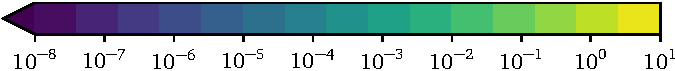
\includegraphics{resultsInterpolationPointwise_4}\\[2mm]%
  \subcaptionbox{%
    $\bspl{\*l,\*i}{p}\vphantom{\bspl[\nak]{\*l,\*i}{p}}$%
  }[48mm]{%
    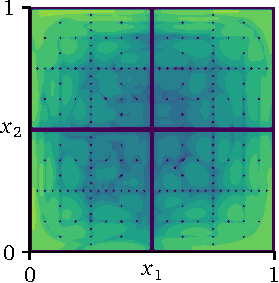
\includegraphics{resultsInterpolationPointwise_1}%
  }%
  \hfill%
  \subcaptionbox{%
    $\bspl[\nak]{\*l,\*i}{p}$%
  }[48mm]{%
    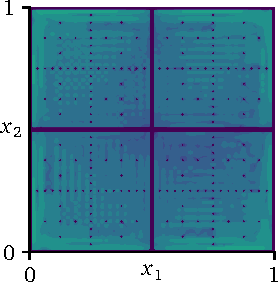
\includegraphics{resultsInterpolationPointwise_2}%
  }%
  \hfill%
  \subcaptionbox{%
    $\bspl[\modified]{\*l,\*i}{p}$%
  }[48mm]{%
    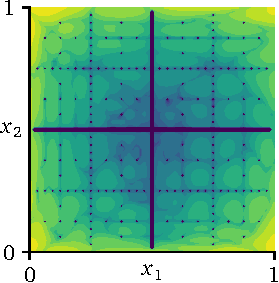
\includegraphics{resultsInterpolationPointwise_3}%
  }%
  \caption[Pointwise interpolation error for the GoP function]{%
    Pointwise interpolation error
    $\abs{\objfun(\*x) - \sgintp(\*x)}$ on a logarithmic scale
    for the bivariate GoP function ($d = 2$)
    using different hierarchical basis functions
    $\basis{\*l,\*i}$ \emph{(left, center, right)} of degree $p = 3$ on
    the regular sparse grid $\regsgset{n}{d}$ of level $n = 7$.%
  }%
  \label{fig:resultsInterpolationErrorPointwise}%
\end{figure}

\vspace*{-0.3em}

\paragraph{Decay of surpluses}

In the piecewise linear case ($p = 1$),
the hierarchical surpluses $\surplus{\*l,\*i}$
can be represented as the $\Ltwo$ inner product of
the corresponding hat function $\bspl{\*l,\*i}{1}$ with the
second mixed derivative
$\partialderiv[2d]{\partialdiff x_1^2 \dotsm \partialdiff x_d^2}{\objfun}$
of the objective function $\objfun$,
if $\*l \ge \*1$ and if this derivative exists and is continuous
(see \cref{eq:surplusIntegral}).
Consequently, one can prove that
$\abs{\surplus{\*l,\*i}} \le 2^{-d} 2^{-2\normone{\*l}}
\normLinftyscaled{
  \partialderiv[2d]{\partialdiff x_1^2 \dotsm \partialdiff x_d^2}{\objfun}
}$ \cite{Bungartz04Sparse},
i.e., the absolute values of the hierarchical surpluses
decay  in quadratic order with the level sum $\normone{\*l}$.
This relation can be used to estimate the convergent range
of the corresponding interpolation error (\cref{%
  fig:resultsInterpolationErrorTestFunctions,%
  fig:resultsInterpolationErrorBasisFunctions%
}).
A generalization of this estimate to higher B-spline degrees $p > 1$
is not straightforward, as the surpluses $\surplus{\*l,\*i}$
then also depend on function values $\objfun(\gp{\*l',\*i'})$ at
grid points of higher levels $\*l' \ge \*l$.

The decay of surpluses can be seen in \cref{fig:resultsDecaySurpluses},
which shows the mean absolute value of surpluses corresponding to
grid points grouped by their level sum $\normone{\*l}$.
Due to the dependency of coarse-level surpluses on high-level grid points
for $p > 1$,
we have to fix the level $n$ of the regular sparse grid for this analysis.
\Cref{fig:resultsDecaySurpluses} suggests that the
absolute value of the surpluses decays with order $p + 1$ for
B-spline degree $p$, although no theoretical evidence
is known to support this claim.
Higher B-spline degrees seem to imply that
$\abs{\surplus{\*l,\*i}}$ generally increases, if $\normone{\*l}$ is
in the preasymptotic range.

\begin{figure}
  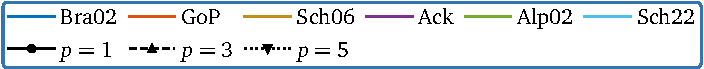
\includegraphics{resultsInterpolationLegend_1}\\[2mm]%
  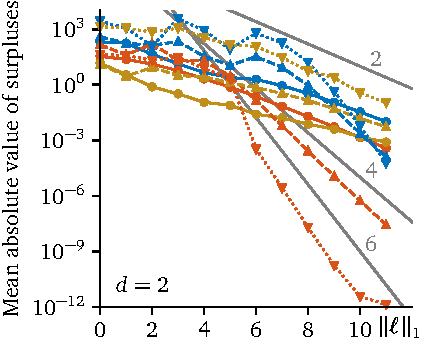
\includegraphics{resultsInterpolation_1}%
  \hfill%
  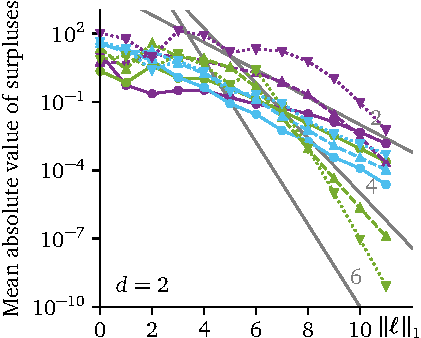
\includegraphics{resultsInterpolation_3}%
  \caption[Decay of surpluses for different test functions]{%
    Mean absolute value of surpluses by level sum $\normone{\*l}$
    \vspace{-0.05em}%
    for different test functions $\objfun$ \emph{(colors)}
    using hierarchical not-a-knot B-splines
    $\bspl[\nak]{\*l,\*i}{p}$ of different degrees $p$
    \emph{(line styles/markers)} on
    the regular sparse grid $\regsgset{n}{d}$ of level $n = 11$.%
  }%
  \label{fig:resultsDecaySurpluses}%
\end{figure}



\subsection{Complexity of Hierarchization}
\label{sec:543complexity}

In \cref{chap:40algorithms}, we introduced a number of new
hierarchical spline bases with the aim to reduce the complexity
of algorithms with the key example of hierarchization.
In the following, we study the suitability of the new bases
to achieve this goal \cite{Valentin18Fundamental}.

\paragraph{Complexity of fundamental splines}

\Cref{fig:complexityFundamental} compares the hierarchization complexity of
modified hierarchical B-splines $\bspl[\modified]{\*l,\*i}{p}$ with the new
modified hierarchical fundamental splines $\bspl[\fs,\modified]{\*l,\*i}{p}$
as measured on a laptop with Intel Core i5-4300U.
For the modified hierarchical B-spline basis,
we solve a linear system of size $\ngp \times \ngp$,
for which Gaussian elimination takes
$\landauTheta{\ngp^3}$ time and $\landauTheta{\ngp^2}$ memory for
$\ngp \to \infty$ (where $\ngp$ is the number of sparse grid points and
$d$ is assumed to be constant).
More sophisticated methods to solve linear systems
are not able to significantly
reduce this complexity without any further assumptions on the system matrix
$\intpmat$ (e.g., symmetry, positive definiteness, or bandedness).
As $\ngp$ grows,
the space needed to store an $\ngp \times \ngp$ matrix quickly exceeds
the available memory.

For the modified hierarchical fundamental splines,
we can use the \bfs algorithm presented in \cref{sec:44spatAdaptiveBFS}.
\bfs works in quadratic time $\landauO{\ngp^2}$, but more importantly,
it works in linear space $\landauO{\ngp}$.
Both can be seen very well in \cref{fig:complexityFundamental}:
The computation time drops from cubic to quadratic complexity for fundamental splines
and the consumed memory is reduced from quadratic to linear complexity.

\begin{figure}
  
\includegraphics{complexityFundamental_3}\\[2mm]%
  \subcaptionbox{%
    Computation time%
  }[72mm]{%
    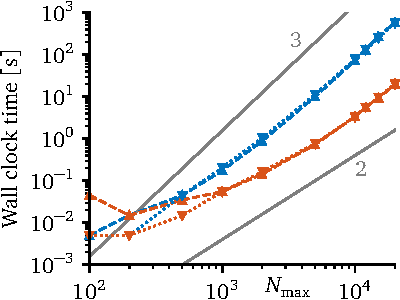
\includegraphics{complexityFundamental_1}%
  }%
  \hfill%
  \subcaptionbox{%
    Memory consumption%
  }[72mm]{%
    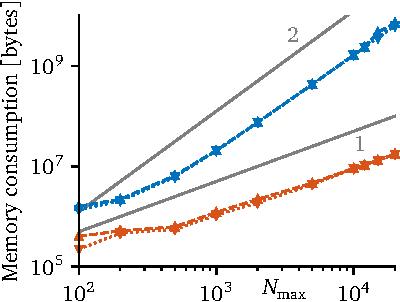
\includegraphics{complexityFundamental_2}%
  }%
  \caption[Complexity of fundamental splines]{%
    Computation time and memory consumption of hierarchization
    with modified hierarchical B-splines
    $\bspl[\modified]{\*l,\*i}{p}$ \emph{\textcolor{C0}{(blue)}} and
    \vspace*{-0.3em}%
    modified hierarchical fundamental splines
    $\bspl[\fs,\modified]{\*l,\*i}{p}$ \emph{\textcolor{C1}{(red)}}
    of degrees $p = 3$ and $p = 5$
    on the spatially adaptive sparse grids generated by the criterion of
    Novak--Ritter for the optimization of Ack with $d = 4$ and
    $\ngpMax$ grid points.
    Adapted from \cite{Valentin18Fundamental}.%
  }%
  \label{fig:complexityFundamental}%
\end{figure}

\paragraph{Complexity of weakly fundamental splines}

It is not straightforward to include weakly fundamental splines
in \cref{fig:complexityFundamental} as we have to insert missing
chain points to apply the unidirectional principle
(see \cref{sec:45spatAdaptiveUP}).
As this increases the number of necessary evaluations of $\objfun$,
a comparison of computation times with standard B-splines would be skewed.
Instead, we study in \cref{fig:complexityWeaklyFundamental}
the number of grid points that have to be inserted
to ensure the correctness of the unidirectional principle.
As we have seen in \cref{sec:453chains}
(cf.\ \cref{fig:chainInsertionBSpline}),
inserting all chains needed for standard hierarchical B-splines
often results in a full grid, which suffers from the curse of dimensionality.
%
\begin{figure}
  
\includegraphics{complexityWeaklyFundamental_4}\\[2mm]%
  \subcaptionbox{%
    $\gamma = 0.05$%
  }[48mm]{%
    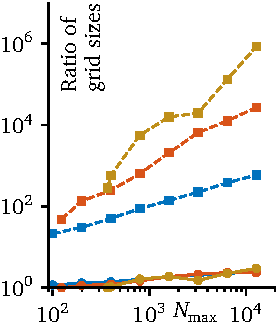
\includegraphics{complexityWeaklyFundamental_1}%
  }%
  \hfill%
  \subcaptionbox{%
    $\gamma = 0.15$%
  }[48mm]{%
    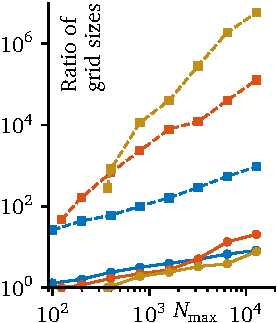
\includegraphics{complexityWeaklyFundamental_2}%
  }%
  \hfill%
  \subcaptionbox{%
    $\gamma = 0.25$%
  }[48mm]{%
    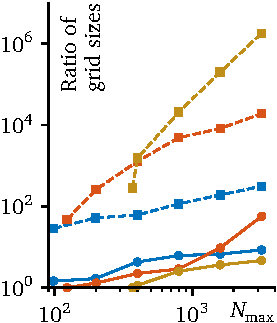
\includegraphics{complexityWeaklyFundamental_3}%
  }%
  \caption[Complexity of weakly fundamental splines]{%
    Total number of grid points after inserting all missing chains
    for cubic weakly fundamental not-a-knot splines
    $\bspl[\wfs,\nak]{\*l,\*i}{p}$ \emph{($p = 3$, solid lines),}
    and after inserting all missing full grid points \emph{(dashed).}
    Shown are the ratios of the resulting grid sizes to the
    initial grid sizes before inserting points.
    The initial grids are the spatially adaptive sparse grids generated
    by the criterion of Novak--Ritter for the optimization of Ack with
    different dimensionalities \emph{(colors)},
    different adaptivity parameters $\gamma$ \emph{(left, center, right),}
    and $\ngpMax$ grid points.%
  }%
  \label{fig:complexityWeaklyFundamental}%
\end{figure}%
%
This can be seen in \cref{fig:complexityWeaklyFundamental}
for hierarchical not-a-knot B-splines (dashed lines).
By inserting all full grid points,
the number of grid points increases by several orders of magnitude:
If the initial grid has $\ngpMax = \num{10000}$ points,
then the grid size increases roughly by the factor $10^2$ for $d = 2$,
$10^4$ for $d = 3$, and $10^6$ for $d = 4$,
resulting in computationally infeasible
grids with $10^6$, $10^8$, and $10^{10}$ points, respectively.
If we instead only insert the missing chain points needed for the
hierarchical weakly fundamental not-a-knot basis
(solid lines, cf.\ \cref{fig:chainInsertionWeaklyFundamentalSpline}),
then the number of grid points increases only slightly.
For grids that have a low adaptivity (which correspond
to low adaptivity parameters $\gamma$ in the Novak--Ritter criterion,
see \cref{sec:521novakRitter}), the grid size only increases by the
factor of two.
For highly-adaptive grids
(corresponding to large $\gamma$),
the number of necessary chain grid points increases significantly.



\subsection{Optimality Gap}
\label{sec:542optimization}

\paragraph{Optimality gaps and displacements}

With the method described in \cref{sec:52method},
we find approximations $\xoptappr$ of the
global minimum $\xopt$ of some objective function $\objfun$
using optimization of a B-spline surrogate $\sgintp$ of $\objfun$
on sparse grids.
Obviously, the more accurate the sparse grid surrogate is,
the better the approximation $\xoptappr$ will be.
In the following plots,
we show the optimality gaps $\objfun(\xoptappr) - \objfun(\xopt)$
in terms of function values.%
\footnote{%
  In order to calculate the optimality gap,
  it is crucial to determine $\objfun(\xopt)$ as exact as possible.
  Otherwise, the optimality gap might either not converge to zero
  or it might even become negative.%
}
The results are sensitive to even small displacements
of the objective function, i.e.,
the results may change for the
function $\*x \mapsto \objfun(\*x - \*a)$
instead of $\*x \mapsto \objfun(\*x)$ for $\*x \in \clint{\*0, \*1}$
and some small $\*a \in \real^d$.%
\footnote{%
  By using the formulas in \cref{chap:a20testProblems},
  all test functions $\objfun$ in \cref{sec:53testProblems}
  can be extended such that they can be evaluated at $\*x - \*a$
  for all $\*x \in \clint{\*0, \*1}$, if $\*a \in \real^d$ is small enough.
  Note that we set $a_t$ to zero if a non-zero displacement in
  the $t$-th component would change the location of the global minimum.%
}
Therefore, the optimization for each of the
data points for \cref{%
  fig:resultsOptimizationUnconstrainedTestFunctions,%
  fig:resultsOptimizationConstrainedTestFunctions%
}
was repeated five times with replacements $\*a$
whose entries $a_t$ were independent and identically distributed Gaussian
pseudo-random numbers with zero mean and a standard deviation of $0.01$.
The optimality gaps shown in the figures of this section were computed
as the mean of the five runs to increase confidence in the results.

\paragraph{Unconstrained optimization}

\Cref{fig:resultsOptimizationUnconstrainedTestFunctions}
shows the optimality gaps for different test functions $\objfun$
over the number $\ngpMax$ of allowed evaluations of $\objfun$.
For the continuously differentiable functions
Bra02, GoP\punctfix{,} Ack, and Alp02
in $d = 2$ dimensions (top row),
the optimization of the corresponding cubic B-spline surrogates (solid lines)
performs significantly better than using piecewise linear basis functions
(dashed lines).
The reason is two-fold:
First, by using higher-order basis functions, the surrogates are more accurate
in general as seen in the discussion of the interpolation error in
\cref{sec:541interpolation}.
Second, the availability of surrogate gradients accelerates the
convergence of the employed optimization methods.
For some test functions, B-splines give better results than even
the direct optimization of the objective function (dotted lines).

\begin{figure}
  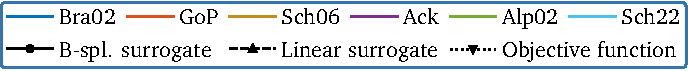
\includegraphics{resultsOptimizationLegend_1}\\[2mm]%
  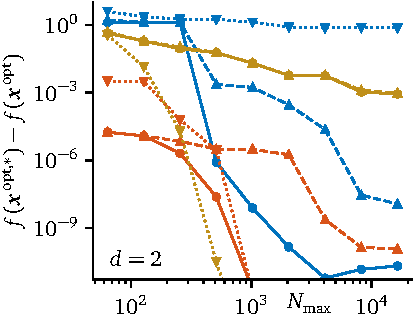
\includegraphics{resultsOptimizationUnconstrained_1}%
  \hfill%
  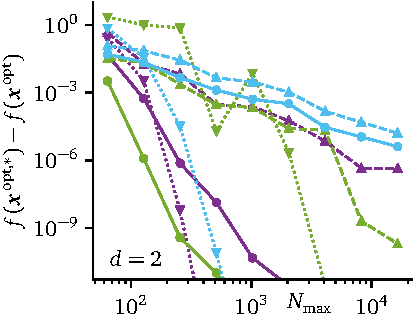
\includegraphics{resultsOptimizationUnconstrained_2}%
  \\[2mm]%
  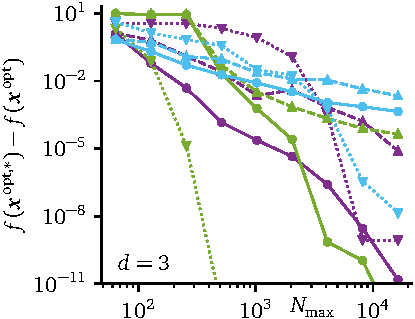
\includegraphics{resultsOptimizationUnconstrained_3}%
  \hfill%
  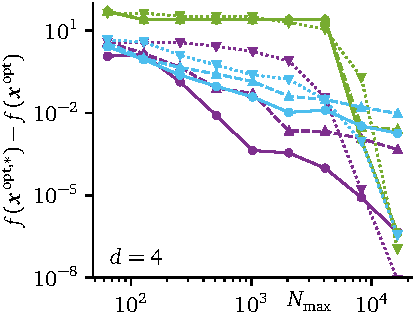
\includegraphics{resultsOptimizationUnconstrained_4}%
  \\[2mm]%
  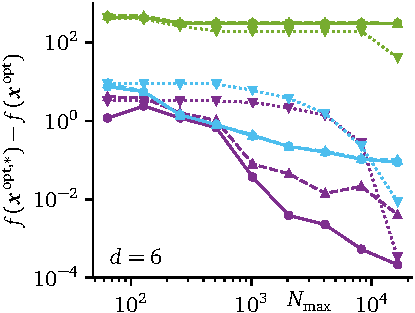
\includegraphics{resultsOptimizationUnconstrained_5}%
  \hfill%
  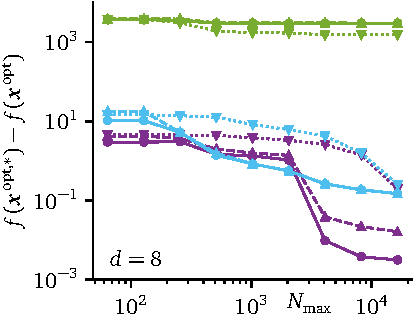
\includegraphics{resultsOptimizationUnconstrained_6}%
  \caption[Optimality gaps for different objective functions (unconstrained)]{%
    Optimality gaps $\objfun(\xoptappr) - \objfun(\xopt)$ between
    the function value at the approximated optimum $\xoptappr$ and
    the minimal function value at the actual optimum $\xopt$
    over the number $\ngpMax$ of objective function evaluations
    for different unconstrained
    objective functions $\objfun$ \emph{(colors).}
    Shown are the optimization results of the B-spline surrogate
    \emph{(solid lines),}
    the optimization results of the piecewise linear surrogate
    \emph{(dashed),} and
    the optimization results of the actual objective function
    \emph{(dotted)} as described in \cref{sec:52method}.%
  }%
  \label{fig:resultsOptimizationUnconstrainedTestFunctions}%
\end{figure}

For the test functions Sch06 and Sch22 with discontinuous derivatives,
the advantage of higher-order B-splines is not as evident (Sch22) or
does not even exist (Sch06).
However, in low dimensions, i.e., $d \le 4$, B-splines
achieve a slight advantage compared to the piecewise linear basis
for the Sch22 function.
In higher dimensionalities, i.e., $d \ge 6$ (bottom row),
convergence visibly slows down for all methods shown in
\cref{fig:resultsOptimizationUnconstrainedTestFunctions},
although for some objective functions, B-splines are still able
to perform better than the comparison methods
(most notably for the Ack function).

\paragraph{Constrained optimization}

\Cref{fig:resultsOptimizationConstrainedTestFunctions}
shows the result for the two constrained optimization problems.
The objective function value $\objfun(\xoptappr)$
at the approximated optimum $\xoptappr$ should not only
be as small as possible, but $\xoptappr$ should also be feasible, i.e.,
$\ineqconfun(\xoptappr) \le \*0$.
Hence, we also plot the maximal violation
$\norm[\infty]{\nonnegpart{\ineqconfun(\xoptappr)}}$
of the constraints in the respective optimal points $\xoptappr$.

\begin{figure}
  
\includegraphics{resultsOptimizationLegend_2}\\[2mm]%
  \subcaptionbox{%
    G08%
  }[72mm]{%
    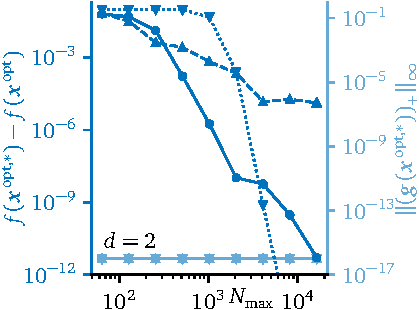
\includegraphics{resultsOptimizationConstrained_1}%
  }%
  \hfill%
  \subcaptionbox{%
    G04Sq%
  }[72mm]{%
    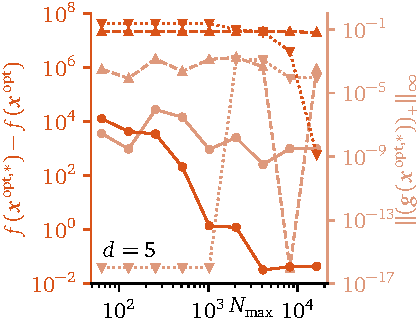
\includegraphics{resultsOptimizationConstrained_2}%
  }%
  \caption[Optimality gaps for different objective functions (constrained)]{%
    Optimality gaps $\objfun(\xoptappr) - \objfun(\xopt)$ between
    the function value at the approximated optimum $\xoptappr$ and
    the minimal function value at the actual optimum $\xopt$
    over the number $\ngpMax$ of objective function evaluations
    for different constrained optimization problems
    \emph{(dark, left vertical axes).}
    In addition to the lines of
    \cref{fig:resultsOptimizationUnconstrainedTestFunctions},
    the constraint violation
    $\norm[\infty]{\nonnegpart{\ineqconfun(\xoptappr)}}$
    at the approximated optimum $\xoptappr$ is plotted
    \emph{(light, right vertical axes).}%
  }%
  \label{fig:resultsOptimizationConstrainedTestFunctions}%
\end{figure}

For the bivariate G08 problem, the hierarchical B-splines surrogates
perform better than the direct gradient-free optimization of the problem
for $\ngpMax \le 3500$ objective function evaluations
and better than the piecewise linear surrogate for $\ngpMax \ge 300$
objective function evaluations.
All calculated points are feasible.%
\footnote{%
  For plotting reasons,
  \cref{fig:resultsOptimizationConstrainedTestFunctions} shows
  $\max(\norm[\infty]{\nonnegpart{\ineqconfun(\xoptappr)}}, 10^{-16})$
  instead of the true constraint violation.%
}

The range of the objective function of the five-dimensional G04Sq problem
is larger than the range of G08.
This results in generally higher optimality gaps
$\objfun(\xoptappr) - \objfun(\xopt)$ as we do not normalize
with respect to the range.
B-splines achieve good approximations $\xoptappr$
of $\xopt$ already for $\ngpMax = 1000$ with an optimality gap of
around one.
Both comparison methods show optimality gaps that are
seven orders of magnitude higher.

Additionally, the corresponding values of constraint violation
are between $10^{-10}$ and $10^{-6}$, i.e.,
the constraints are numerically met.
In contrast, the optimizers struggle more for
the comparison methods (optimization of the linear surrogate and
of the objective function) to meet the constraints,
as the values of the constraint violation partly exceed $10^{-3}$.
The availability of gradients seems to allow the constrained optimization
methods to better enforce the feasibility of the
resulting points $\xoptappr$.

Note that while the results look already promising for the B-spline surrogate
method, these results could still be improved upon.
The Novak--Ritter criterion used to generate the
spatially adaptive sparse grids does not take the constraints into account.
Consequently, many sparse grid points are created outside the feasible domain.
By modifying the criterion to prefer points that are in a neighborhood of
the feasible domain, the quality of the interpolant
close to potential optima should increase.
